% econ — process & memory map  (companion to ECON_ARCHITECTURE.md §11.1)
% Standalone TikZ figure for papers / slides.
% Build:  pdflatex econ-architecture.tex
% Deps:   only `standalone` + `tikz` (TeX Live / MiKTeX default).
\documentclass[border=12pt]{standalone}
\usepackage{tikz}
\usetikzlibrary{positioning,arrows.meta,fit,backgrounds}
\begin{document}
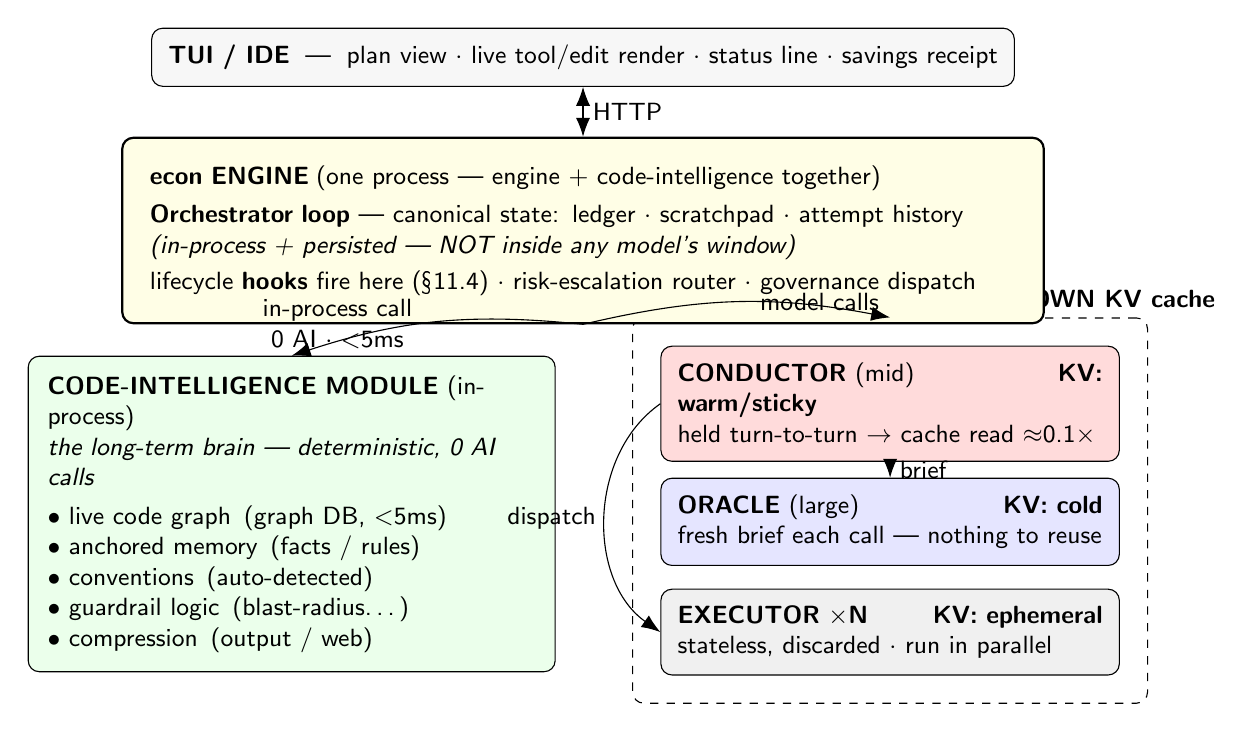
\begin{tikzpicture}[
    font=\small\sffamily,
    >={Latex[length=2.4mm]},
    box/.style   ={draw, rounded corners, align=left, inner sep=6pt, fill=black!3},
    engine/.style={draw, thick, rounded corners, align=left, inner sep=10pt,
                   fill=yellow!10, text width=11cm},
    comp/.style  ={draw, rounded corners, align=left, inner sep=7pt,
                   fill=green!8, text width=6.2cm},
    warm/.style  ={draw, rounded corners, align=left, inner sep=6pt,
                   fill=red!14,  text width=5.4cm},
    cold/.style  ={draw, rounded corners, align=left, inner sep=6pt,
                   fill=blue!10, text width=5.4cm},
    eph/.style   ={draw, rounded corners, align=left, inner sep=6pt,
                   fill=black!6, text width=5.4cm},
  ]

  % --- top: the UI -------------------------------------------------------
  \node[box] (tui) at (0,8.4)
    {\textbf{TUI / IDE} \;\textemdash\; plan view $\cdot$ live tool/edit render $\cdot$ status line $\cdot$ savings receipt};

  % --- the engine --------------------------------------------------------
  \node[engine] (engine) at (0,6.2)
    {\textbf{econ ENGINE}\;(one process \textemdash\ engine + code-intelligence together)\\[3pt]
     \textbf{Orchestrator loop} \textemdash\ canonical state: ledger $\cdot$ scratchpad $\cdot$ attempt history\\
     \emph{(in-process + persisted \textemdash\ NOT inside any model's window)}\\[2pt]
     lifecycle \textbf{hooks} fire here (\S11.4) $\cdot$ risk-escalation router $\cdot$ governance dispatch};

  % --- left: the deterministic brain ------------------------------------
  \node[comp] (side) at (-3.7,2.6)
    {\textbf{CODE-INTELLIGENCE MODULE} (in-process)\\
     \emph{the long-term brain \textemdash\ deterministic, 0 AI calls}\\[3pt]
     $\bullet$ live code graph \,(graph DB, $<$5ms)\\
     $\bullet$ anchored memory \,(facts / rules)\\
     $\bullet$ conventions \,(auto-detected)\\
     $\bullet$ guardrail logic \,(blast-radius\ldots)\\
     $\bullet$ compression \,(output / web)};

  % --- right: the model endpoints, each with its own KV cache -----------
  \node[warm] (cond) at (3.9,4.0)
    {\textbf{CONDUCTOR} (mid) \hfill \textbf{KV: warm/sticky}\\
     held turn-to-turn $\rightarrow$ cache read $\approx$0.1$\times$};
  \node[cold] (orac) at (3.9,2.5)
    {\textbf{ORACLE} (large) \hfill \textbf{KV: cold}\\
     fresh brief each call \textemdash\ nothing to reuse};
  \node[eph]  (exec) at (3.9,1.1)
    {\textbf{EXECUTOR $\times$N} \hfill \textbf{KV: ephemeral}\\
     stateless, discarded $\cdot$ run in parallel};

  \begin{scope}[on background layer]
    \node[draw, dashed, rounded corners, inner sep=10pt, fill=white,
          fit=(cond)(orac)(exec),
          label={[font=\small\sffamily\bfseries]above:MODEL ENDPOINTS \textemdash\ each owns its OWN KV cache}]
          (models) {};
  \end{scope}

  % --- wiring ------------------------------------------------------------
  \draw[<->] (tui) -- node[right]{HTTP} (engine);
  \draw[->] (engine.south) to[bend right=12]
        node[left, align=center, pos=0.55]{in-process call\\0 AI $\cdot$ $<$5ms} (side.north);
  \draw[->] (engine.south) to[bend left=12]
        node[right, pos=0.55]{model calls} (models.north);

  \draw[->] (cond.south) -- node[right]{brief} (orac.north);
  \draw[->] (cond.west) to[bend right=55] node[left, pos=0.5]{dispatch} (exec.west);

\end{tikzpicture}
\end{document}
